\section*{Abstract}

Diese Arbeit praesentiert das Design eines Roboters, der autonom ein Wegentz durchqueren kann und dabei zufaellig platzierte Hindernisse erkennen kann. Dazu wurden die Teilfunktionen der Roboters definiert und durch Prototyping entwickelt.

Es wurde ein Roboter designed, der den Linien auf einem Wegenetz folgen kann, sich darauf um die eigene Achse drehen kann und Hindernisse selbstaendig erkennt und einordnet. Bewegliche Hindernisse auf dem Wegenetz koennen sicher angehoben und wieder zurueckgestellt werden.

\begin{figure}[H]
\centering
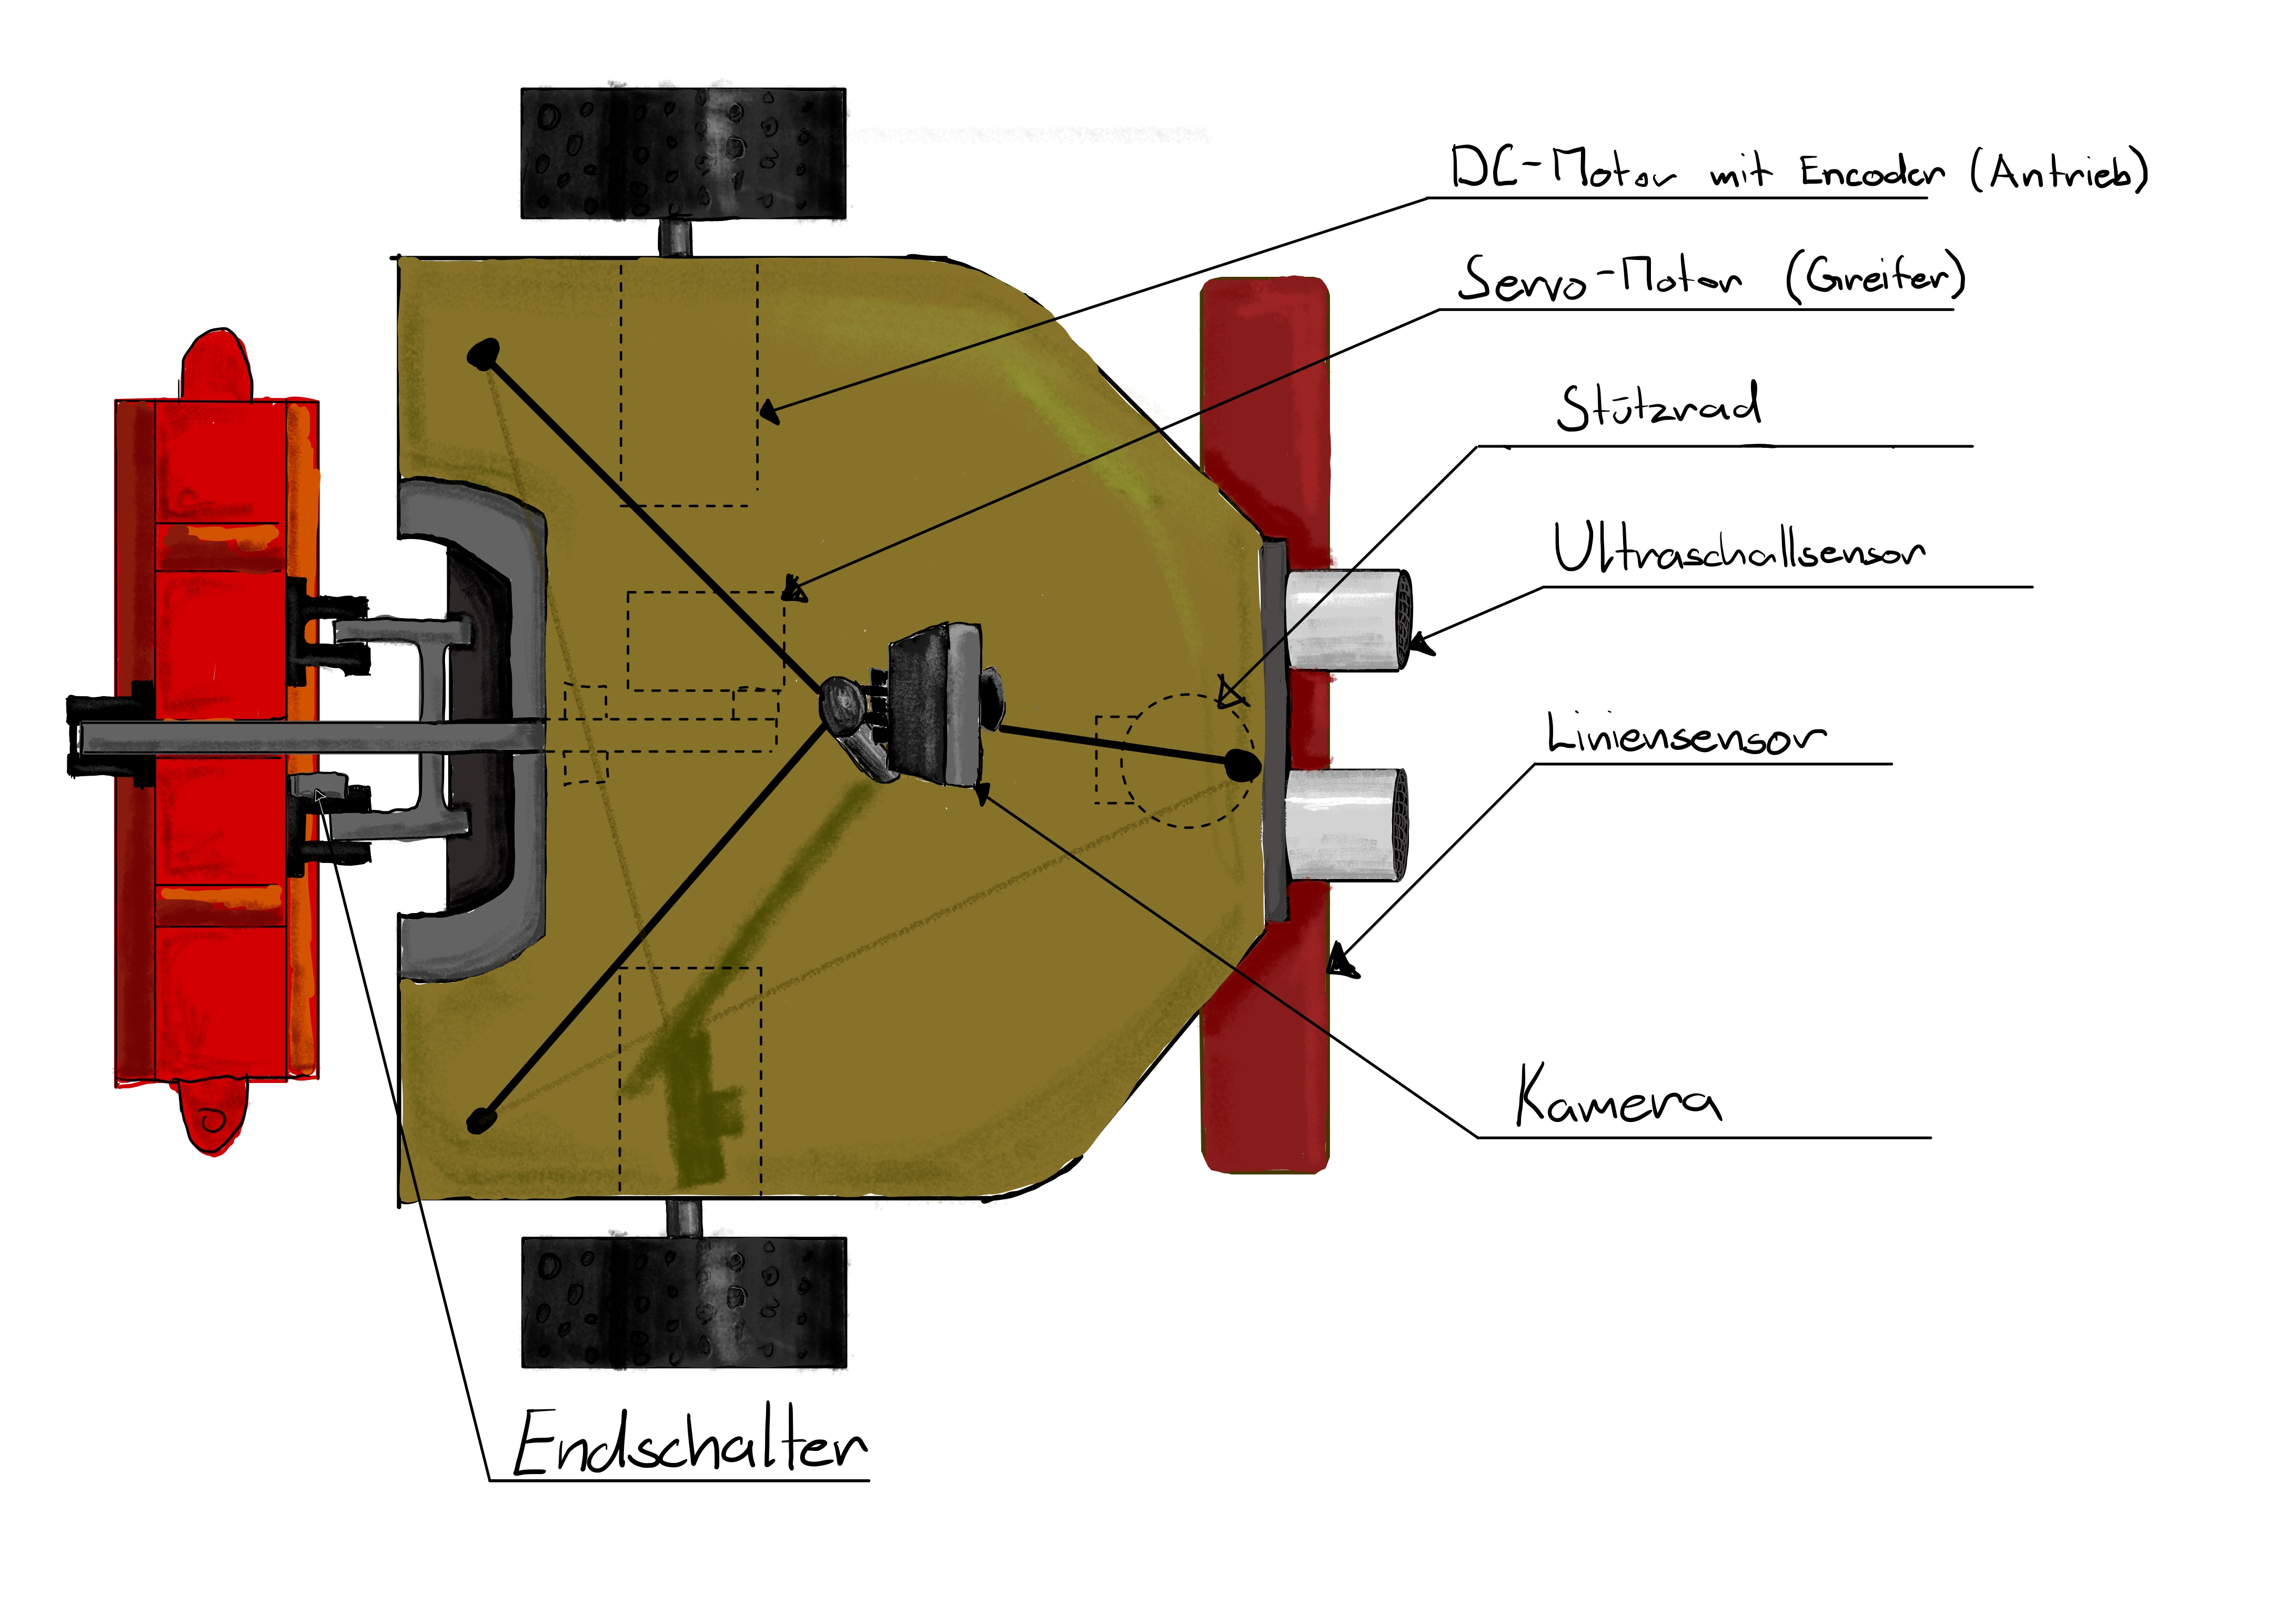
\includegraphics[width=0.7\textwidth]{assets/gesamtkonzept/Skizze-Fahrzeugkonzept-Beschriftet.jpg}
\caption{Konzeptskizze Gesamtkonzept}
\label{fig:robot_concept-scetch_labeld-abstract}
\end{figure}

Der Roboter wird das Wegenetz auf drei Raedern durchfahren, wobei zwei davon mit Motoren betrieben werden. Ein Liniensensor bestehend aus Fototransistoren wird eingesetzt, damit der Roboter die Linien des Wegenetzweks nicht verlaesst.

Die Hebervorrichtung, die der Roboter braucht, um bewegliche Hindernisse zu beseitigen, wird mit einem Greifer umgesetzt. Ein Ultraschallsensor detektiert, sobald sich eine Barriere in der Naehe befindet, damit sich der Greifer langsam darauf zu bewegen kann. Sobald die Endschalter am Greifer betaetigt werden, greift dieser zu. Durch die doppelte Hindernisdetektierung ist der Roboter zuverlaessig und durch die Konstruktion des Greifers, kann das Hindernis sicher gefasst werden, auch falls sich dieses schraeg auf der Linie befindet.

Hindernisse werden mit einer Kamera und Bilderkennung erkannt, damit der Roboter weiss, welche Wege befahrbar sind. Es kann Zeit eingespart werden, da die Hindernisse aus der Distanz geprueft werden.

Um die Machbarkeit zu simulieren wurde ein Simulator programmiert. Dieser stellt dar, wie der Roboter sich durch das Wegenetz fortbewegt und misst die Zeit. Zusaetzlich dient er als Grundlage zur Navigation im richtigen Roboter.

Das finale Design des autonomen Roboters bietet eine effiziente und sichere Loesung, um das Wegenetz zu durchqueren. Es ist eine zuverlaessige Grundlage fuer die Umsetzung in PREN 2.



